%=============================================================================
%  report_ieee14_switching_decision_basis_en.tex
%  English report: the decision basis of the IEEE-14 1-SG / 4-IBR GFL/GFM
%  mode-switching supervisor.
%
%  Answers five questions:
%    Q1 why a switching event promotes one or two converters, not all four;
%    Q2 from what value the damping margin is computed, how, and why that value;
%    Q3 the short-circuit ratio at the converter buses once the SG is tripped;
%    Q4 what happens if all four become grid-forming, and whether a strong grid
%       is not desirable;
%    Q5 the two-term voltage/frequency index is judged too narrow, and three
%       additional indices are designed.
%
%  EVIDENCE BASE
%  - Every measured number is read out of a named artefact of the delivered
%    result set (output/diagnostics/ieee14_gfm_lock_compare_zeta/, built by
%    scripts/reporting/run_ieee14_gfm_lock_comparison.m) or out of a named
%    source line of the production code. Nothing is interpolated or estimated.
%  - Where a quantity is a derived diagnostic rather than a production result,
%    it is labelled as such at the point of use.
%  - The two indices in Section 10 are a DESIGN PROPOSAL. They are not
%    implemented and no run in this repository consumes them. They are labelled
%    PROPOSED at every use, and no measured result in this report depends on
%    them.
%
%  BUILD:  xelatex report_ieee14_switching_decision_basis_en.tex   (twice)
%=============================================================================
\documentclass[12pt,a4paper]{article}

\usepackage{graphicx,amsmath,amssymb,float,caption,hyperref,fancyhdr}
\usepackage{amsthm}
\usepackage{newtxtext,newtxmath}
\newtheorem{proposition}{Proposition}
\theoremstyle{remark}
\newtheorem{remark}{Remark}
\usepackage{geometry,booktabs,tabularx,array,longtable,microtype}
\usepackage{xcolor}
\usepackage{enumitem}
\usepackage{tikz}
\usetikzlibrary{arrows.meta,positioning,calc,patterns,shapes.geometric}
\geometry{margin=1in}
\setlength{\headheight}{14.5pt}
\pagestyle{fancy}
\fancyhf{}
\lhead{IEEE-14 GFL/GFM switching: decision basis}
\rhead{\thepage}
\renewcommand{\headrulewidth}{0.4pt}
\renewcommand{\arraystretch}{1.14}
\emergencystretch=1.5em

\definecolor{navy}{RGB}{25,55,95}
\definecolor{ok}{RGB}{0,110,70}
\definecolor{no}{RGB}{170,40,35}
\definecolor{warn}{RGB}{175,110,0}
\definecolor{pale}{RGB}{240,244,249}

\newcommand{\pu}{\,\mathrm{pu}}
\newcommand{\Ibr}{\mathrm{IBR}}
\newcommand{\zmin}{\zeta_{\min}}
\newcommand{\zworst}{\zeta_{\mathrm{worst}}}
\newcommand{\greq}{\gamma_{\mathrm{req}}}
\newcommand{\Ssev}{S}
\newcommand{\code}[1]{\texttt{\small #1}}
\newcommand{\measured}{\textcolor{ok}{\textbf{[measured]}}}
\newcommand{\derived}{\textcolor{warn}{\textbf{[derived]}}}
\newcommand{\proposed}{\textcolor{navy}{\textbf{[proposed]}}}

\title{\bfseries Admissibility, damping margin and island grid strength\\[2pt]
in the IEEE-14 grid-forming switching study\\[8pt]
\large Why a switching event promotes one or two converters,\\
and three proposed switching indices}
\author{In-house power system analysis toolkit}
\date{}

\begin{document}
\maketitle
\thispagestyle{fancy}

\begin{abstract}
\noindent
The IEEE-14 study network carries one synchronous machine at bus~1 and four
dual-mode converters at buses 2, 3, 6 and 8, each able to run grid-following
(GFL) or grid-forming (GFM). When the machine trips, a supervisor decides how
many converters to promote and which ones. This report establishes, from the
delivered code and the delivered result caches, that the promotion count is not
chosen by a stability objective and not by ``more is safer'': it is the
\emph{minimum-cardinality strict superset} of the currently forming set that
appears in a pre-computed, authenticated admissibility table, and that table is
\emph{not monotone} in the count. Of the fifteen possible forming sets, only seven
are admissible; \emph{every} three-converter set has no equilibrium at all
(coupled-Newton residual $3.28$--$3.61\times10^{2}$). The acceptance criterion is
a robust damping-ratio floor $\zmin = 0.05$ evaluated at three frozen
finite-difference steps, and the all-four set is admissible but is the least
damped of the seven ($\zworst = 0.1223$ against $0.2549$--$0.2676$). The island
short-circuit ratio at the converter buses stays between $2.30$ and $2.73$ in
every islanded window --- below the WECC strong-grid floor of $3$ on $98.61\%$
of all converter-samples, and below it on $100\%$ of the post-trip and
post-reclose windows. The delivered adaptive chronology promotes one unit at a
time, holds two for most of the islanded window and reaches four only when
nothing smaller is admissible. Finally, the report measures five failure modes
of the present two-term voltage/frequency switching index on the delivered run
--- among them that its frequency half is \emph{identical} across all four
converters for all $3679$ samples --- and designs three additional indices that
each enter their own non-tradeable condition rather than a re-weighted scalar.
\end{abstract}

\tableofcontents
\clearpage

%=============================================================================
\section{Scope, questions and evidence base}
%=============================================================================

\subsection{The five questions}

\begin{enumerate}[leftmargin=1.6em,itemsep=2pt]
\item \textbf{Promotion count.} In the latest model code, why does a switching
      event not place every converter in grid-forming mode, but select only one
      or two?
\item \textbf{Damping margin.} From what quantity is the margin computed, how is
      it computed, and why is that the quantity that is used?
\item \textbf{Island grid strength.} What is the short-circuit ratio (SCR) at
      the converter buses once the synchronous machine is tripped out?
\item \textbf{All four forming.} What happens if all four converters form, why is
      that undesirable, and is a strong grid not a good thing?
\item \textbf{Switching index.} The index that drives switching today uses only
      voltage and frequency. That is judged too narrow and capable of producing
      false decisions. Three further indices are designed.
\end{enumerate}

\subsection{What ``proof'' means here, and what it does not}

This report proves statements of two different kinds, and keeps them apart.

\paragraph{Model-internal statements} are proved by reading the production code
that the delivered run executes. ``The promotion is the minimum-cardinality
strict superset'' is a statement of this kind: it is a property of
\code{select\_support\_augmentation\_candidate.m} and of the table the run
consumes, and it holds for every run of this code, not only for the delivered
one.

\paragraph{Trajectory statements} are proved by measurement on a named artefact.
``The island SCR is $2.3$ once the machine is out'' is a statement of this kind:
it is true of \code{adaptive\_250s.mat} and of the network and dispatch that
cache was built from, and it is not claimed to be universal.

No statement in this report is proved by argument alone. Where a mechanism is
offered as an explanation rather than as a measurement, it is marked as an
explanation at the point of use, and Section~12 lists what is \emph{not}
claimed.

\subsection{Artefacts}

\begin{table}[H]
\centering
\small
\begin{tabularx}{\textwidth}{@{}lX@{}}
\toprule
\textbf{Artefact} & \textbf{Role in this report}\\
\midrule
\code{+stability/ts\_simulate\_ibr\_hybrid.m} &
  the supervisor: severity formation, hysteresis, dwell, and the call into
  candidate selection and the support transaction.\\
\code{+stability/select\_support\_augmentation\_candidate.m} &
  the ranking rule that turns ``severity says more support is needed'' into one
  named forming set.\\
\code{+stability/ibr\_candidate\_evaluate.m} &
  the acceptance criterion: equilibrium, KCL, full-KCL small-signal spectrum and
  the robust damping-ratio gate.\\
\code{+stability/ibr\_scr\_metrics.m} &
  the short-circuit-ratio metric and its gate.\\
\code{+stability/agsi\_reference\_terms.m} &
  the reference sub-indices published beside the run, including the three the
  decision does not consume.\\
\code{+cases/case\_ieee14\_1sg\_4ibr\_auto\_vsg.m} &
  the case, its dispatch contract and its frozen selector contract
  (\code{case\_data.selector}, \code{:168--174}).\\
\code{run\_ieee14\_gfm\_lock\_comparison.m} &
  the six-arm study and the shared option set every arm starts from.\\
\code{ieee14\_gfm\_lock\_compare\_zeta/adaptive\_250s.mat} &
  the delivered 250\,s adaptive chronology. Every trajectory number below is
  read from this file.\\
\code{ieee14\_gfm\_lock\_compare\_zeta/summary.mat} &
  the admissibility enumeration of Section~\ref{sec:admissibility}.\\
\code{docs/project/defects/2026-08-14-all4-gfm-commit-outside-basin.md} &
  the measured root cause of the all-four failure mode.\\
\bottomrule
\end{tabularx}
\caption{Artefacts this report reads. No file is written by the reading.}
\end{table}

\subsection{The delivered result, for orientation}

\begin{table}[H]
\centering
\small
\begin{tabularx}{\textwidth}{@{}lrX@{}}
\toprule
\textbf{Quantity} & \textbf{Value} & \textbf{Source}\\
\midrule
horizon reached & $250.000000$ s & \code{result.t(end)}\\
accepted samples & $3679$ & \code{numel(result.t)}\\
rejected steps / attempts & $161$ / $3824$ & \code{rejected\_steps}, \code{ts\_step\_attempts}\\
max accepted KCL residual & $9.972081\times10^{-9}$ & \code{max(accepted\_residual\_per\_step)}\\
terminal $f_{\mathrm{COI}}$ & $60.000001128$ Hz & \code{coi\_frequency\_Hz(end)}\\
SG reclose & $159.2519$ s, \code{SUCCESS} & \code{actual\_reclose\_time}\\
reference handback complete & $173.1271$ s, \code{C1\_COMPLETE} & \code{handback\_complete\_time}\\
\bottomrule
\end{tabularx}
\caption{The delivered adaptive chronology. These seven values are the
project's regression gate for this result set.}
\end{table}

%=============================================================================
\section{The studied system and what the supervisor is for}
%=============================================================================

\subsection{The network and the resources}

The case is \code{case\_profile} $=$ \code{'eecon49\_figure4'} on the IEEE-14
network, resolved to \code{ibr\_model\_id} $=$ \code{'eecon49\_dual'}. The
resource table is fixed and its order is the only identity the selector uses:

\begin{table}[H]
\centering
\small
\begin{tabular}{@{}clrlrrl@{}}
\toprule
\textbf{Index} & \textbf{Id} & \textbf{Bus} & \textbf{Type} & \textbf{Base (MVA)} & \textbf{Initial} & \textbf{Model}\\
\midrule
1 & SG1  & 1 & synchronous & 615 & online & \code{sg\_emf6}\\
2 & IBR2 & 2 & converter   & 100 & GFL    & \code{eecon49\_dual}\\
3 & IBR3 & 3 & converter   & 100 & GFL    & \code{eecon49\_dual}\\
4 & IBR6 & 6 & converter   & 100 & GFL    & \code{eecon49\_dual}\\
5 & IBR8 & 8 & converter   & 100 & GFL    & \code{eecon49\_dual}\\
\bottomrule
\end{tabular}
\caption{The resource table. Bus numbers and device names are never decision
keys; resource-table indices are.}
\end{table}

The machine contributes $H = 2.5$\,s and $D = 1.0\pu$ in the delivered option
set. Each converter carries a filter $L_f = 0.15\pu$, $R_f = 0.015\pu$, a DC
link $C_{dc} = 0.10$, and a current ceiling $I_{\max} = 1.2\pu$ on the common
100\,MVA base. The grid-forming branch is a virtual synchronous machine with
swing coefficient $M = 0.08$ and damping coefficient $D_v = 20.0$; the
grid-following branch is a PLL-based current controller with
$k_{p,\mathrm{PLL}} = 1.20$, $k_{i,\mathrm{PLL}} = 5.00$. The same $D_v$
coefficient fixes both the $P$--$f$ droop and the swing damping, which is a
property of this single-coefficient VSG and not a modelling oversight.

\subsection{What the machine carries, and what the trip hands over}

At the pre-event power flow the machine supplies $1.3319\pu$ and the four
converters together supply $1.3176\pu$, against a total load of $2.59\pu$ of
active power and $0.735\pu$ of reactive power. The case's own dispatch contract
records the consequence of opening the machine breaker as
\code{deficit\_MW} $= 133.1904$ and \code{lost\_sg\_Q\_MVAr} $= -19.5666$.
\measured

Opened at $t = 20$\,s, that breaker leaves an energized island whose voltage is
formed by converters alone, and it obliges the supervisor to answer two separate
questions: \emph{when} is more forming support required, and \emph{which}
converters should provide it. The code answers them in two different places, and
that separation is the subject of Section~\ref{sec:pipeline}.

\subsection{The delivered switching history}

\begin{table}[H]
\centering
\small
\begin{tabular}{@{}rlrll@{}}
\toprule
$t$ (s) & \textbf{event} & \textbf{forming set} & \textbf{transition} & \textbf{variant}\\
\midrule
$0.0000$    & initial              & $\{\}$               & all GFL, SG online & ---\\
$20.0000$   & SG trip              & $\{2\}$              & IBR2 $\to$ GFM     & ---\\
$22.0887$   & support augment      & $\{2,4\}$            & $+$IBR6            & unconditioned\\
$25.3026$   & support release      & $\{2\}$              & $-$IBR6            & unconditioned\\
$50.0000$   & load step $+20\%$    & $\{2\}$              & ---                & ---\\
$51.3403$   & support augment      & $\{2,4\}$            & $+$IBR6            & unconditioned\\
$53.3795$   & support augment      & $\{2,3,4,5\}$        & $+$IBR3, $+$IBR8   & \textbf{conditioned}\\
$85.0000$   & fault, bus 9         & $\{2,3,4,5\}$        & ---                & ---\\
$85.1500$   & fault cleared        & $\{2,3,4,5\}$        & ---                & ---\\
$110.0000$  & line 6--13 trip      & $\{2,3,4,5\}$        & ---                & ---\\
$145.0000$  & topology restored, reclose requested & $\{2,3,4,5\}$ & --- & ---\\
$146.2782$  & support release      & $\{2\}$              & $-$IBR3,\,IBR6,\,IBR8 & unconditioned\\
$148.2811$  & support augment      & $\{2,4\}$            & $+$IBR6            & unconditioned\\
$152.4017$  & support release      & $\{2\}$              & $-$IBR6            & unconditioned\\
$159.2519$  & \textbf{SG reclose}  & $\{2\}$              & \code{SUCCESS}     & ---\\
$173.1271$  & handback, IBR2 $\to$ GFL & $\{\}$           & ---                & ---\\
\bottomrule
\end{tabular}
\caption{Every mode transaction of the delivered adaptive chronology, read from
\code{result.device\_modes\_history} and \code{result.event\_log}.
\measured}
\label{tab:timeline}
\end{table}

Read the ``transition'' column as the answer to Q1 in its most literal form.
Five augment or release events occur in 250\,s, and \emph{every one of them moves
by one or two units}. The set never jumps from $\{2\}$ to $\{2,3,4,5\}$ in a
single transaction. Section~\ref{sec:count} shows that this is structural, not
incidental.

%=============================================================================
\section{The decision pipeline}\label{sec:pipeline}
%=============================================================================

The supervisor is three stages in series, and each stage can only refuse. No
stage can overrule a refusal by another.

\begin{figure}[H]
\centering
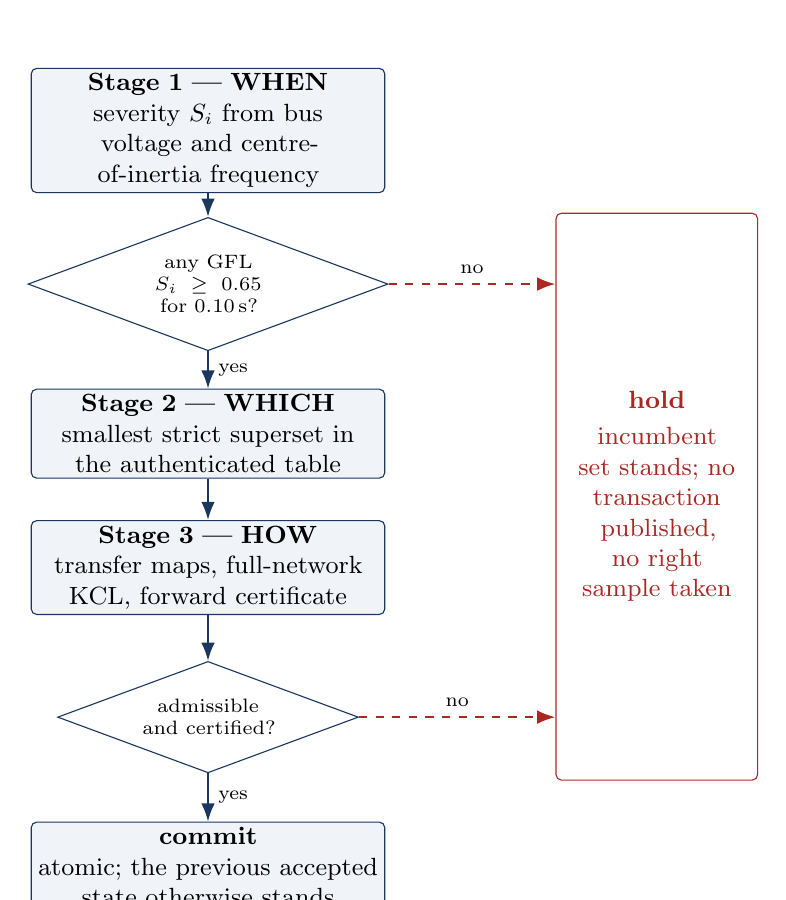
\begin{tikzpicture}[font=\small,>=Latex,
  box/.style={draw=navy,rounded corners=2pt,fill=pale,minimum height=8mm,
              text width=4.35cm,align=center,inner sep=2pt},
  gate/.style={draw=navy,diamond,aspect=2.7,fill=white,text width=2.6cm,
               align=center,inner sep=0pt,font=\scriptsize},
  arr/.style={->,thick,draw=navy},
  ref/.style={->,thick,draw=no,dashed}]
\node[box] (s1) at (0,0) {\textbf{Stage 1 --- WHEN}\\severity $\Ssev_i$ from bus
  voltage and centre-of-inertia frequency};
\node[gate] (g1) at (0,-1.95) {any GFL\\$\Ssev_i \ge 0.65$\\for $0.10$\,s?};
\node[box] (s2) at (0,-3.85) {\textbf{Stage 2 --- WHICH}\\smallest strict
  superset in the authenticated table};
\node[box] (s3) at (0,-5.55) {\textbf{Stage 3 --- HOW}\\transfer maps,
  full-network KCL, forward certificate};
\node[gate] (g2) at (0,-7.45) {admissible\\and certified?};
\node[box] (cm) at (0,-9.35) {\textbf{commit}\\atomic; the previous accepted
  state otherwise stands};
\node[draw=no,rounded corners=2pt,fill=white,minimum height=72mm,
      text width=2.35cm,align=center,inner sep=3pt] (hold) at (5.7,-4.65)
  {\color{no}\textbf{hold}\\[2pt] incumbent set stands; no transaction published,
   no right sample taken};
\draw[arr] (s1)--(g1);
\draw[arr] (g1)--node[right,font=\scriptsize]{yes}(s2);
\draw[arr] (s2)--(s3);
\draw[arr] (s3)--(g2);
\draw[arr] (g2)--node[right,font=\scriptsize]{yes}(cm);
\draw[ref] (g1.east)--node[above,font=\scriptsize]{no}(g1.east -| hold.west);
\draw[ref] (g2.east)--node[above,font=\scriptsize]{no}(g2.east -| hold.west);
\end{tikzpicture}
\caption{The three stages. Stage 1 is a new decision every sample; stages 2 and
3 are lookups and tests against evidence frozen before the run started.}
\label{fig:pipeline}
\end{figure}

\subsection{Stage 1 --- when support is requested}

For every online switchable converter the driver forms

\begin{equation}
\Ssev_i \;=\; \operatorname{sat}\!\left(\tfrac{1}{2}J_{V,i} + \tfrac{1}{2}J_f\right),
\qquad
J_{V,i} = \frac{|V_i - V_{i,\text{healthy}}|}{0.10},
\qquad
J_f = \frac{|f_{\mathrm{COI}} - 60|}{0.50},
\label{eq:severity}
\end{equation}

with $\operatorname{sat}(x) = \min(1,\max(0,x))$
\code{(ts\_simulate\_ibr\_hybrid.m:3631)}, bases $0.10\pu$ and $0.50$\,Hz fixed at
\code{:1675--1677}, and $V_{i,\text{healthy}}$ the pre-event power-flow voltage
of that converter's own bus. The promotion and release conditions are

\begin{equation}
\text{augment} \;=\; \bigl|\{\,i \in \text{GFL} : \Ssev_i \ge 0.65\,\}\bigr| > 0,
\qquad
\text{release} \;=\; \forall i,\; \Ssev_i < 0.35,
\label{eq:triggers}
\end{equation}

sustained for $T_{d,\mathrm{on}} = 0.10$\,s and $T_{d,\mathrm{off}} = 1.00$\,s
respectively \code{(:852--900)}, with the thresholds set at \code{:1664--1667}.
Three properties of \eqref{eq:triggers} matter later:

\begin{itemize}[leftmargin=1.4em,itemsep=1pt]
\item the augment term is an \code{any} over the \emph{followers}. The index
      therefore asks ``is a grid-following converter under stress?'', not ``is
      the system stable?'' and not ``which converter is the cause?''.
\item the release term is an \code{all}. Hysteresis is asymmetric on purpose:
      support is added on the first follower in trouble and withdrawn only when
      every converter is comfortable for a full second.
\item no term of \eqref{eq:severity} is a stability quantity. Feasibility,
      small-signal margin, current limits and reference ownership are all
      elsewhere, and Section~\ref{sec:indices} argues that this is correct ---
      but that the \emph{set} of quantities entering Stage 1 is too small.
\end{itemize}

\subsection{Stage 2 --- which converters}

Stage 1 produces a direction, never a set. The set comes from a table of
candidate configurations computed before the simulation starts
(\code{ibr\_selector\_table}), and the runtime rule is
\code{select\_support\_augmentation\_candidate}:

\begin{proposition}[Minimum-cardinality admissible superset]
\label{prop:superset}
Let $\mathcal{F}$ be the forming set at the decision instant and $\mathcal{T}$
the set of table rows with \code{feasible} and \code{ready\_to\_commit} both
true. The returned destination is the row $c \in \mathcal{T}$ minimising, in
order: (i) $|\mathrm{selected}(c)|$; (ii) $-\mathrm{margin}(c)$; (iii) the
selected index tuple lexicographically; (iv) the reference index --- subject to
$\mathcal{F} \subsetneq \mathrm{selected}(c)$, i.e.\ the destination must be a
\emph{strict} superset of the current set
\code{(select\_support\_augmentation\_candidate.m:54--58, 101--112)}. If no such
row exists the function returns \code{found=false} and the supervisor holds its
incumbent set; it never fabricates a candidate and never relaxes a gate.
\end{proposition}

Two consequences are immediate and are the direct answer to Q1.

\begin{enumerate}[leftmargin=1.6em,itemsep=2pt]
\item \textbf{The cardinality objective is a minimum, not a maximum.} Nothing in
      Proposition~\ref{prop:superset} rewards adding converters. A three-unit
      destination is chosen over a two-unit destination only when no two-unit
      strict superset is admissible.
\item \textbf{The choice is not a free re-selection.} Because the destination
      must contain the current set, the supervisor cannot answer ``the island
      needs four formers'' by promoting four units at once from one former; it
      can only add to what it has, and it adds as few as the table permits.
\end{enumerate}

\subsection{Stage 3 --- how the transition is applied}

The mode change passes through device-owned transfer maps, then a full-network
Kirchhoff solve at the new operating point, then --- because the option is
enabled in this study --- a forward simulation of the would-be committed state
with the same integration kernel over a horizon derived from the destination's
own settling time. A refusal is atomic: no right sample is published, the
previous accepted state stands, and a named identifier plus a lockout is
recorded. Over the delivered 250\,s the certificate was consulted at four
transactions, and it changed the outcome at one of them
(Table~\ref{tab:timeline}, $t = 53.3795$: the untouched arrival was rejected and
the conditioned variant committed at a peak excursion of $15.495^{\circ}$).
\measured

%=============================================================================
\section{The admissibility enumeration}\label{sec:admissibility}
%=============================================================================

Stage 2 has nothing to choose from unless a table exists, and the table is not a
formality. Five converters, four of them switchable, admit $2^4 - 1 = 15$
non-empty forming sets. The project computes every one of them.

\begin{table}[H]
\centering
\small
\begin{tabular}{@{}clrrcl@{}}
\toprule
\textbf{Set} & \textbf{Ref} & $\omega$ (rad/s) & $\mathrm{margin}$ & $\zworst$ & \textbf{Outcome}\\
\midrule
$\{5\}$        & 5 & $-0.155437$ & $+0.055437$ & $0.2676$ & admissible\\
$\{4\}$        & 4 & $-0.252025$ & $+0.152025$ & $0.2629$ & admissible\\
$\{3\}$        & 3 & $-0.316711$ & $+0.216711$ & $0.2618$ & admissible\\
$\{2\}$        & 2 & $-0.328014$ & $+0.228014$ & $0.2569$ & admissible\\
$\{2,4\}$      & 2 & $-0.561723$ & $+0.461723$ & $0.2549$ & admissible\\
$\{3,4\}$      & 3 & $\mathbf{-0.568138}$ & $\mathbf{+0.468138}$ & $0.2560$ & admissible (most damped)\\
\midrule
$\{2,3\}$      & --- & --- & --- & --- & no equilibrium: IBR6 violates a limit\\
$\{2,5\}$      & --- & --- & --- & --- & no equilibrium: IBR6 violates a limit\\
$\{3,5\}$      & --- & --- & --- & --- & no equilibrium: IBR6 violates a limit\\
$\{4,5\}$      & --- & --- & --- & --- & no equilibrium: IBR3 violates a limit\\
\midrule
$\{2,3,4\}$    & --- & --- & --- & --- & no equilibrium, residual $3.279\times10^{2}$\\
$\{2,3,5\}$    & --- & --- & --- & --- & no equilibrium, residual $3.605\times10^{2}$\\
$\{2,4,5\}$    & --- & --- & --- & --- & no equilibrium, residual $3.561\times10^{2}$\\
$\{3,4,5\}$    & --- & --- & --- & --- & no equilibrium, residual $3.346\times10^{2}$\\
\midrule
$\{2,3,4,5\}$  & 2 & $-0.482909$ & $+0.382909$ & $\mathbf{0.1223}$ & admissible, least damped\\
\bottomrule
\end{tabular}
\caption{The complete SG-off admissibility enumeration, read from
\code{summary.shared.sg\_off\_candidates} in
\code{ieee14\_gfm\_lock\_compare\_zeta/summary.mat}. Seven of fifteen sets are
admissible. This is a \emph{base-load table, frozen before candidate evaluation};
the load-level sensitivity of Section~\ref{sec:allfour} is a separate measurement
at $+20\%$ load and does not modify these rows.
$\omega$ is the least damped member of the frozen finite-difference set,
$\omega = \max(\texttt{cand.fd\_omegas})$
\code{(ibr\_candidate\_evaluate.m:447)}, not the value at a single step;
$\mathrm{margin} = -\omega - \greq$; $\zworst$ is the worst damping ratio over the
physical decision spectrum, minimised over the same three finite-difference
members. \measured}
\label{tab:adm}
\end{table}

\begin{figure}[H]
\centering
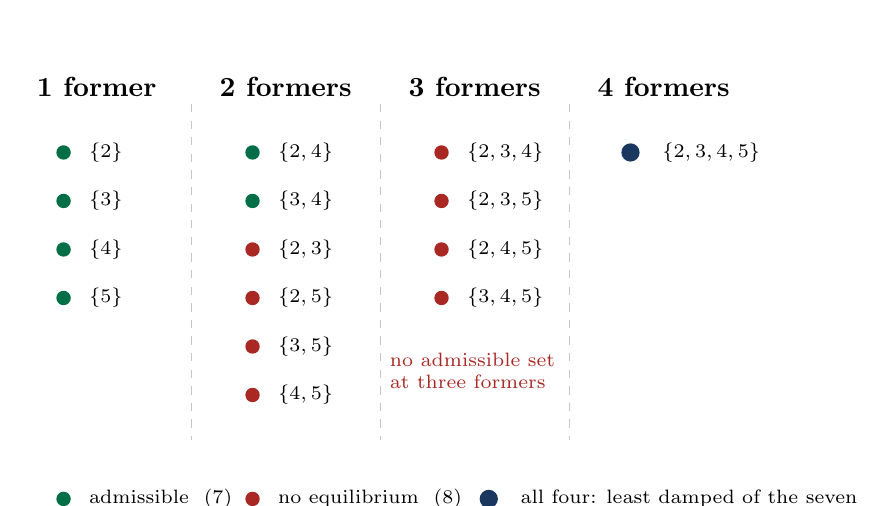
\begin{tikzpicture}[font=\scriptsize,x=1cm,y=0.88cm]
\node[font=\bfseries] at (0.42,0.95) {1 former};
\node[font=\bfseries] at (2.82,0.95) {2 formers};
\node[font=\bfseries] at (5.22,0.95) {3 formers};
\node[font=\bfseries] at (7.62,0.95) {4 formers};
\foreach \x in {1.62,4.02,6.42} \draw[gray!45,dashed] (\x,0.7)--(\x,-4.15);
% one former
\fill[ok] (0,0) circle (2.6pt);      \node[anchor=west] at (0.2,0)      {$\{2\}$};
\fill[ok] (0,-0.7) circle (2.6pt);   \node[anchor=west] at (0.2,-0.7)   {$\{3\}$};
\fill[ok] (0,-1.4) circle (2.6pt);   \node[anchor=west] at (0.2,-1.4)   {$\{4\}$};
\fill[ok] (0,-2.1) circle (2.6pt);   \node[anchor=west] at (0.2,-2.1)   {$\{5\}$};
% two formers
\fill[ok] (2.4,0) circle (2.6pt);    \node[anchor=west] at (2.6,0)      {$\{2,4\}$};
\fill[ok] (2.4,-0.7) circle (2.6pt); \node[anchor=west] at (2.6,-0.7)   {$\{3,4\}$};
\fill[no] (2.4,-1.4) circle (2.6pt); \node[anchor=west] at (2.6,-1.4)   {$\{2,3\}$};
\fill[no] (2.4,-2.1) circle (2.6pt); \node[anchor=west] at (2.6,-2.1)   {$\{2,5\}$};
\fill[no] (2.4,-2.8) circle (2.6pt); \node[anchor=west] at (2.6,-2.8)   {$\{3,5\}$};
\fill[no] (2.4,-3.5) circle (2.6pt); \node[anchor=west] at (2.6,-3.5)   {$\{4,5\}$};
% three formers
\fill[no] (4.8,0) circle (2.6pt);    \node[anchor=west] at (5.0,0)      {$\{2,3,4\}$};
\fill[no] (4.8,-0.7) circle (2.6pt); \node[anchor=west] at (5.0,-0.7)   {$\{2,3,5\}$};
\fill[no] (4.8,-1.4) circle (2.6pt); \node[anchor=west] at (5.0,-1.4)   {$\{2,4,5\}$};
\fill[no] (4.8,-2.1) circle (2.6pt); \node[anchor=west] at (5.0,-2.1)   {$\{3,4,5\}$};
% four formers
\fill[navy] (7.2,0) circle (3.3pt);  \node[anchor=west] at (7.48,0)     {$\{2,3,4,5\}$};
% annotation
\node[anchor=north west,align=left,text=no] at (4.02,-2.75)
  {no admissible set\\at three formers};
% legend
\fill[ok] (0,-5.0) circle (2.6pt);
\node[anchor=west] at (0.2,-5.0) {admissible \ (7)};
\fill[no] (2.4,-5.0) circle (2.6pt);
\node[anchor=west] at (2.6,-5.0) {no equilibrium \ (8)};
\fill[navy] (5.4,-5.0) circle (3.3pt);
\node[anchor=west] at (5.68,-5.0) {all four: least damped of the seven};
\end{tikzpicture}
\caption{The admissibility map. Feasibility is \emph{not} monotone in the number
of forming converters: every admissible set sits below or above the three-unit
row, never on it.}
\label{fig:map}
\end{figure}

\subsection{What the enumeration proves}

\begin{enumerate}[leftmargin=1.6em,itemsep=2.5pt]
\item \textbf{``More forming units'' is not a monotone improvement, and the
      project measured this rather than assuming it.} The middle of the map is
      empty. Three forming converters is not a compromise between two and four;
      it is a configuration for which the coupled Newton finds no operating
      point at all, at any of the four ways of choosing the three.
\item \textbf{The reason is the sharing problem, not the number.} Each of the
      eight infeasible rows fails for a mechanical reason: either a converter
      left in grid-following is asked to violate an operating limit
      ($\{2,3\}$, $\{2,5\}$, $\{3,5\}$, $\{4,5\}$), or the four-way power balance
      has no solution (the four three-unit sets). In both families the failure is
      reported by name, not by a low margin.
\item \textbf{The all-four set is admissible but is the outlier.} Its worst
      damping ratio, $0.1223$, is less than half of every other admissible set's.
      Section~\ref{sec:damping} shows where that number comes from and why it is
      the right thing to gate on.
\end{enumerate}

\begin{remark}[Why a pre-computed table rather than an on-line search]
A candidate is admitted only after its own equilibrium is solved and its own
full-KCL spectrum is assembled at three perturbation sizes. That costs seconds
per candidate and must not sit inside an accepted time step. Pre-computing the
whole universe also makes the runtime decision a pure lookup of evidence the run
can no longer influence, which is what allows Proposition~\ref{prop:superset} to
be stated about the code rather than about a particular trajectory.
\end{remark}

%=============================================================================
\section{The damping margin: how it is computed, and why this value}
\label{sec:damping}
%=============================================================================

\subsection{The computation, step by step}

For each candidate set the evaluator
(\code{+stability/ibr\_candidate\_evaluate.m}) runs the following chain. No step
is skipped, and a failure at any step stops the evaluation with a named
identifier.

\begin{enumerate}[leftmargin=1.7em,itemsep=3pt]
\item \textbf{Freeze the criterion.} $\zmin$ is read from the case's own
      contract, \code{case\_data.selector.zeta\_min\_damping}, not from the
      caller, and is validated to lie in $(0,1)$ \code{(:83--93)}. For this case
      $\zmin = 0.05$.
\item \textbf{Solve the destination equilibrium.} The candidate's exact mode
      assignment is built into the device set and the hybrid state, then solved
      by the coupled Newton with tolerance $10^{-8}$ and 300 iterations
      \code{(:314, :326)}. The machine breaker is held open throughout, because
      the selector owns the post-trip configuration contract and evaluating a
      candidate with the machine closed would certify a different physical
      system \code{(:220--228)}.
\item \textbf{Enforce the network equations.} The physical all-row KCL residual
      must satisfy $\lVert \cdot\rVert \le 10^{-6}$
      \code{(:340--345)}. Measured residuals for the admissible rows are
      $3.6\times10^{-15}$ to $1.4\times10^{-14}$. \measured
\item \textbf{Assemble the decision spectrum.} The full-KCL composite
      state-space model is built at the accepted equilibrium with the exact
      input $u_{eq}$, event context and active-state index set \code{(:355--395)}.
      The network-angle gauge coordinate is removed by a centre-of-inertia
      $T$-matrix, and no eigenvalue is deleted after the eigenvalue call
      \code{(:398--400)}.
\item \textbf{Damping ratio per mode.} Each eigenvalue of the physical decision
      spectrum is reduced to
      \begin{equation}
      \zeta_i = \frac{-\operatorname{Re}\lambda_i}{|\lambda_i|}.
      \label{eq:zeta}
      \end{equation}
      A real negative root gives $\zeta = 1$ and can therefore never be the
      limiting mode. A root \emph{at} the origin has an undefined ratio and is
      mapped to $-\infty$ rather than skipped, so a marginal mode fails any
      positive floor instead of quietly certifying; an empty spectrum likewise
      returns $-\infty$, because no evidence is not evidence of damping
      \code{(:492--516)}.
\item \textbf{Worst over the spectrum, not rightmost.} The reported quantity is
      the minimum of \eqref{eq:zeta} over the whole decision spectrum. This is a
      deliberate departure from reading the margin off
      $\max\operatorname{Re}\lambda$: the worst-damped mode is generally not the
      rightmost one, and reading the ratio off the rightmost eigenvalue would
      miss it \code{(:402--410)}.
\item \textbf{Repeat at three perturbation sizes.} The whole assembly is redone
      at finite-difference steps $\varepsilon \in \{1.5,\,3,\,6\}\times10^{-6}$
      (the audited base times $0.5$, $1$, $2$) and the test is applied at
      \emph{every} member \code{(:412--448)}.
\item \textbf{The gate.} A candidate is admissible when
      \begin{equation}
      \forall \varepsilon \in \mathcal{E}:\quad
      \max\operatorname{Re}\lambda(\varepsilon) < 0
      \quad\text{and}\quad
      \min_i \zeta_i(\varepsilon) \;\ge\; \zmin,
      \label{eq:gate}
      \end{equation}
      that is, all three perturbation sizes must agree both on stability and on
      the ratio floor. Disagreement between them fails closed. For the delivered
      table all three agree, and the reported $\zworst$ is the worst of the
      three.
\end{enumerate}

\subsection{Why a damping \emph{ratio} rather than a decay rate}

The code retains a second, older quantity: $\greq = 0.1$\,rad/s, the reference
decay rate, from which
\begin{equation}
\mathrm{margin} = -\max\operatorname{Re}\lambda - \greq .
\label{eq:margin}
\end{equation}
It is used, and it is used only as the \emph{ordering key} among admissible
candidates \code{(:452--462)}. The distinction is not cosmetic.

An absolute-rate floor asks $\operatorname{Re}\lambda \le -\gamma$ and is
therefore frequency-dependent in effect: the same $\gamma$ is a mild requirement
for a fast mode and an unreachable one for a slow mode. A ratio floor asks the
mode to decay within $\zeta^{-1}$ of a radian and is invariant under a change of
timescale. The two families coincide at exactly one frequency,

\begin{equation}
f^{*} = \frac{\greq}{2\pi\zmin} = \frac{0.1}{2\pi(0.05)} = 0.3183\ \mathrm{Hz},
\label{eq:fstar}
\end{equation}

which is the value the case contract records as \code{equivalence\_frequency\_Hz}.
Away from $f^{*}$ they are different requirements \code{(:402--410)}. This plant
carries modes from roughly $0.02$\,Hz --- the island's electromechanical swing,
slowed by the converters' small inertia --- up to the current-loop band, a span
of more than three decades, so no single absolute rate is a meaningful floor
across it.

\subsection{Why 0.05}

The value is declared by the case, not chosen by the report:

\begin{quote}\small
\begin{tabular}{@{}ll@{}}
\code{acceptance\_criterion} & \code{'damping\_ratio\_floor'}\\
\code{derivation} & \code{'5\% damping at the 1\,Hz electromechanical mode:}\\
                 & \code{zeta >= 0.05 for every mode of the physical decision spectrum'}\\
\code{gamma\_req\_role} & \code{'candidate ordering key and reference decay rate; NOT the acceptance gate'}\\
\code{frozen\_before\_candidate\_eval} & \code{1}\\
\end{tabular}
\end{quote}

One apparent tension in that block should be resolved rather than left for the
reader. The \code{derivation} names a $1$\,Hz electromechanical mode, while
\code{equivalence\_frequency\_Hz} is $0.3183$\,Hz. These are not two claims about
the same thing: $1$\,Hz is the mode at which the classical $5\%$ criterion is
quoted, and $0.3183$\,Hz is the frequency at which a $5\%$ ratio and a
$0.1$\,rad/s rate impose the same requirement, by \eqref{eq:fstar}. The case file
therefore records the origin of the number and the crossover of the two
criterion families separately, and both are needed to read the contract.

The provenance is thus threefold and should be stated plainly. The
\emph{number} $0.05$ is the classical electromechanical damping criterion, used
here as a case-level acceptance floor rather than as a simulation target. The
\emph{scope} --- ``every mode of the physical decision spectrum, at every
perturbation size'' --- is the project's own strengthening: a fleet of modes
with one barely damped member is not rescued by the others being comfortable,
and a margin that exists at one finite-difference step but not at the next is
not a margin. The \emph{frozen} flag makes the criterion a property of the case
file, fixed before any candidate is evaluated, so it cannot be re-tuned to fit an
outcome. This is the mechanism by which a candidate can be admitted at
$\mathrm{margin} < 0$ while being admissible: $\mathrm{margin}$ is a ranking
score against a reference rate, and the gate is the ratio.

\begin{remark}[What the gate is not]
Admissibility is a property of an \emph{equilibrium}, established by
linearisation about it. It says nothing about whether the trajectory arriving at
that equilibrium is inside its region of attraction. Section~\ref{sec:allfour}
shows a measured case in which the equilibrium was admissible and the arrival
was not.
\end{remark}

\subsection{The measured margins}

Table~\ref{tab:adm} gives all seven. Three observations are worth stating
explicitly.

\begin{enumerate}[leftmargin=1.6em,itemsep=2.5pt]
\item \textbf{Every admissible set clears the floor comfortably.} The smallest
      worst ratio is $0.1223$, which is $2.45\times$ the floor of $0.05$. The
      binding constraint in this case is therefore not \eqref{eq:gate} at all;
      it is the existence of an equilibrium at all, which removes $8$ of $15$
      sets.
\item \textbf{The damping ratio and the decay rate disagree, and the gate uses
      the ratio.} On $\omega$, the ordering is
      $\{3,4\} > \{2,4\} > \{2,3,4,5\} > \{2\} > \cdots$, so the all-four set is
      the \emph{second} fastest-decaying admissible set. On $\zworst$ it is the
      worst by a factor of two. The gate follows $\zworst$.
\item \textbf{The two-unit sets are the small-signal optimum, and $\{3,4\}$ is
      the best of them.} $\{3,4\}$ has both the most negative $\omega$
      ($-0.568138$) and a top-tier ratio ($0.2560$). This is why the pinned-arm
      study uses $\{3,4\}$ as the fixed-configuration rival to the adaptive
      policy.
\end{enumerate}

%=============================================================================
\section{Why a switching event promotes one or two, not four}\label{sec:count}
%=============================================================================

\subsection{The mechanism}

Proposition~\ref{prop:superset} fixes the count. Work the delivered timeline
through it.

\begin{table}[H]
\centering
\small
\begin{tabular}{@{}rllll@{}}
\toprule
$t$ (s) & \textbf{incumbent $\mathcal{F}$} & \textbf{candidate supersets} & \textbf{admissible} & \textbf{chosen}\\
\midrule
$22.0887$ & $\{2\}$ & $\{2,3\},\{2,4\},\{2,5\},\{2,3,4\},\{2,3,5\},\{2,4,5\},\{2,3,4,5\}$
          & $\{2,4\},\{2,3,4,5\}$ & $\{2,4\}$\\
$51.3403$ & $\{2\}$ & (as above) & $\{2,4\},\{2,3,4,5\}$ & $\{2,4\}$\\
$53.3795$ & $\{2,4\}$ & $\{2,3,4\},\{2,4,5\},\{2,3,4,5\}$ & $\{2,3,4,5\}$ only & $\{2,3,4,5\}$\\
$148.2811$& $\{2\}$ & (as $22.0887$) & $\{2,4\},\{2,3,4,5\}$ & $\{2,4\}$\\
\bottomrule
\end{tabular}
\caption{Every augment of Table~\ref{tab:timeline} resolved through
Proposition~\ref{prop:superset} using the admissibility of Table~\ref{tab:adm}.}
\label{tab:resolution}
\end{table}

At $t = 22.0887$\,s and $t = 51.3403$\,s two destinations exist and the smaller
one wins on criterion~(i). At $t = 53.3795$\,s --- which is after the $+20\%$
load step, with the island carrying the machine's $133.19$\,MW deficit --- the
two-unit supersets $\{2,3,4\}$ and $\{2,4,5\}$ are among the eight rows with no
equilibrium, so the only admissible destination is the all-four set and criterion
(i) has nothing to choose. \emph{Four forming converters is not a policy
preference; it is the residue of the enumeration after the load step.}

\begin{quote}\small\itshape
The four-unit promotion happens because at $+20\%$ load nothing smaller can be
certified --- not because four was judged better than two.
\end{quote}

\subsection{Correcting the premise, and then answering it}

The question as posed --- ``it never goes to all four, only one or two'' --- is
\emph{partly} true of the delivered chronology and sharply true of the scenario
suite. Both halves should be on the record.

\begin{table}[H]
\centering
\small
\begin{tabular}{@{}llrrl@{}}
\toprule
\textbf{Arm} & \textbf{horizon} & \textbf{peak forming} & \textbf{forming at end} & \textbf{reclose}\\
\midrule
chronology, adaptive      & $250$\,s & $4$ & $0$ & \code{SUCCESS} $159.2519$\,s\\
suite, \code{sg\_load\_step30}  & $150$\,s & $4$ & $4$ & \code{SUCCESS} $81.1500$\,s\\
suite, \code{sg\_fault\_bus9}   & $150$\,s & $\mathbf{2}$ & $0$ & \code{SUCCESS} $81.8627$\,s\\
suite, \code{line\_fault\_9\_14}& $150$\,s & $\mathbf{2}$ & $0$ & \code{SUCCESS} $92.4126$\,s\\
suite, \code{former\_outage}    & $150$\,s & $\mathbf{2}$ & $2$ & \code{SUCCESS} $90.3374$\,s\\
suite, \code{sg\_fault\_cycle160}& $160$\,s & $\mathbf{2}$ & $0$ & \code{SUCCESS} $102.3627$\,s\\
\bottomrule
\end{tabular}
\caption{Peak forming count per delivered arm, read from each arm's
\code{device\_modes\_history}. Four of the five suite arms never exceed two
forming converters; the two arms that reach four are the two that carry a large
load step, for the reason in Table~\ref{tab:resolution}. \measured}
\label{tab:arms}
\end{table}

So the accurate statement is:

\begin{itemize}[leftmargin=1.4em,itemsep=2pt]
\item \emph{Per event}, the promotion is one or two units, always, structurally,
      for the reason proved above. In the delivered chronology the forming count
      takes the values $1 \to 2 \to 1 \to 2 \to 4 \to 1 \to 2 \to 1$ across the
      islanded window, with durations $36.98$\,s, $9.37$\,s and $92.90$\,s for
      one, two and four formers respectively. \measured
\item \emph{Per arm}, four of the five delivered suite arms peak at two. The
      delivered $250$\,s chronology and \code{sg\_load\_step30} reach four, and
      both are the arms with a heavy load step.
\item \emph{In no arm} does the supervisor jump from one former straight to four
      in a single transaction, because no such transaction exists in the table's
      strict-superset relation over one step.
\end{itemize}

\subsection{Why the release is faster than the promotion}

The asymmetry in \eqref{eq:triggers} ($T_{d,\mathrm{on}} = 0.10$\,s against
$T_{d,\mathrm{off}} = 1.00$\,s) is deliberate: add support on the first evidence,
withdraw it only after a second of calm. The measured cost is visible at
$t = 146.2782$\,s, where three devices return to grid-following
$1.28$\,s after the reclose request, and the island runs on one former again
from $152.4017$\,s to the reclose at $159.2519$\,s. That is the design working:
the supervisor is willing to run a thin island while the machine is being pulled
into phase, because a transition during the synchronising window is itself a
risk. \measured

%=============================================================================
\section{Island short-circuit strength after the machine trips}\label{sec:scr}
%=============================================================================

\subsection{How the project defines SCR}

\code{+stability/ibr\_scr\_metrics.m} defines, per online converter,

\begin{equation}
\mathrm{SCR}_i = \frac{S_{sc,i}}{S_{\mathrm{rated},i}},
\qquad
S_{sc,i} = \frac{|V_i|^2}{|Z_{th,ii}|}\,S_{\text{base}},
\qquad
Z_{th,ii} = \left[\,\mathbf{Y}^{-1}\mathbf{e}_i\,\right]_i ,
\label{eq:scr}
\end{equation}

with $\mathbf{Y}$ built from the branch data --- including tap and phase shift,
and bus shunts, but \emph{not} load admittance, so that the result measures
network strength rather than loading --- and with reference buses treated as
grounded so that the Thevenin equivalent is taken with the voltage sources
shorted. The rating is the converter's own MVA base; if it is missing the
evaluation fails closed rather than inferring a rating. The threshold is
$\mathrm{SCR} > 3$, taken from the WECC REGC\_A strong-grid contract, and the
comparison is strict: $\mathrm{SCR} \le 3$ is a refusal.

\subsection{The gate is not applicable to this model family}

This must be stated before any number, because it is easy to mistake a published
diagnostic for an active gate. In \code{ibr\_scr\_metrics.m:266--276} the
screening profile is forced for the project's full-state dual families:

\begin{quote}\small
\code{scr\_profile = 'not\_applicable\_full\_state\_source\_model'}\quad for
\code{model\_id} $\in$ \{\code{eecon49\_dual}, \code{decoupled\_dual}\}
\end{quote}

The consequence is \code{eligible\_for\_scr = false} and \code{pass = true}, with
the recorded reason

\begin{quote}\small\itshape
``SCR threshold not applicable to this full-state model; equilibrium, limits and
full-KCL SSSA remain mandatory''.
\end{quote}

\measured{} --- verified for all four converters on the delivered case: every
\code{per\_resource} entry reports \code{eligible\_for\_scr = 0},
\code{SCR = NaN}, \code{pass = 1}. The reason is sound: the REGC\_A screen exists
for a reduced current-source plant model, whereas \code{eecon49\_dual} carries
the AC filter, the DC link, the PLL/VSG and both control loops as explicit
states, so the weak-grid failure the screen protects against is represented in
the model rather than assumed away. The SCR number is nevertheless a meaningful
\emph{physical} statement about the island, and the run publishes it as a
per-sample diagnostic.

\subsection{The measured island SCR}

\begin{table}[H]
\centering
\small
\begin{tabular}{@{}lrrrrr@{}}
\toprule
\textbf{Window} & $n$ & \textbf{min} & \textbf{mean} & \textbf{max} & \textbf{below 3}\\
\midrule
pre-trip, machine online & $168$ & $2.0892$ & $2.3439$ & $2.4803$ & $100.00\%$\\
post-trip, islanded      & $2760$ & $0.6501$ & $2.3015$ & $2.8147$ & $100.00\%$\\
after the load step      & $3152$ & $1.5411$ & $2.6899$ & $3.2908$ & $95.53\%$\\
fault at bus 9, $85.00$--$85.15$ & $164$ & $0.2944$ & $1.2954$ & $6.6726$ & $97.56\%$\\
line 6--13 out           & $2160$ & $2.0718$ & $2.7319$ & $6.6184$ & $97.96\%$\\
restore to reclose       & $4384$ & $1.8361$ & $2.5914$ & $3.5322$ & $99.64\%$\\
after reclose            & $1928$ & $1.9104$ & $2.3291$ & $2.4833$ & $100.00\%$\\
\midrule
whole run, all four converters & $14716$ & $0.2944$ & $2.5271$ & $6.6726$ & $\mathbf{98.61\%}$\\
\bottomrule
\end{tabular}
\caption{Per-sample SCR at the converter buses, from the run's own
\code{agsi\_reference.scr} diagnostic. Classification
\code{ASSUMED\_DIAGNOSTIC}; the ratio uses each converter's rated MVA on the
system base ($100$\,MVA), and the numerator uses the measured bus voltage of
that sample. \measured}
\label{tab:scr}
\end{table}

\begin{figure}[H]
\centering
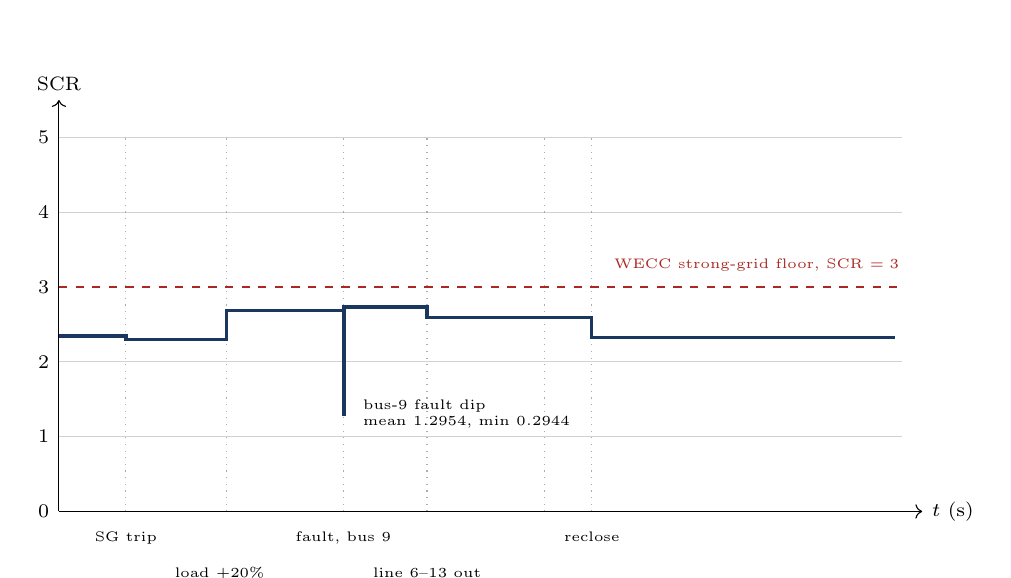
\begin{tikzpicture}[font=\scriptsize,x=0.0425cm,y=0.95cm]
% gridlines and tick labels
\foreach \y in {1,2,4,5} \draw[gray!35] (0,\y)--(252,\y);
\draw[no,thick,dashed] (0,3)--(252,3);
\foreach \y in {0,1,2,3,4,5} \node[left,font=\scriptsize] at (0,\y) {\y};
% axes
\draw[->] (0,0)--(258,0) node[right,font=\scriptsize]{$t$ (s)};
\draw[->] (0,0)--(0,5.5) node[above,font=\scriptsize]{SCR};
% event markers
\foreach \x/\lab in {20/trip,50/load,85/fault,110/line,145/restore,159.25/reclose}
  \draw[gray!65,dotted] (\x,0)--(\x,5);
% window-mean profile (step plot)
\draw[navy,very thick]
  (0,2.3439)--(20,2.3439)--(20,2.3015)--(50,2.3015)--(50,2.6899)
  --(85,2.6899)--(85,1.2954)--(85.15,1.2954)--(85.15,2.7319)
  --(110,2.7319)--(110,2.5914)--(159.25,2.5914)
  --(159.25,2.3291)--(250,2.3291);
% annotations
\node[no,anchor=south west,font=\tiny] at (163,3.08)
  {WECC strong-grid floor, SCR $=3$};
\node[anchor=west,font=\tiny,align=left] at (88,1.30)
  {bus-9 fault dip\\mean $1.2954$, min $0.2944$};
\node[anchor=north,font=\tiny] at (20,-0.14) {SG trip};
\node[anchor=north,font=\tiny] at (85,-0.14) {fault, bus 9};
\node[anchor=north,font=\tiny] at (159.25,-0.14) {reclose};
\node[anchor=north,font=\tiny] at (48,-0.62) {load $+20\%$};
\node[anchor=north,font=\tiny] at (110,-0.62) {line 6--13 out};
\end{tikzpicture}
\caption{The mean SCR across the four converters, as a step plot of the
per-window means of Table~\ref{tab:scr}. The dashed line is the WECC strong-grid
floor. The island never leaves the weak-grid region, and the deepest excursion
coincides with the fault, not with the machine trip.}
\label{fig:scrplot}
\end{figure}

\subsection{Reading the number}

\begin{enumerate}[leftmargin=1.6em,itemsep=2.5pt]
\item \textbf{The machine trip barely moves the SCR.} $2.3439 \to 2.3015$ on the
      window mean. This is not an error: $Z_{th}$ in \eqref{eq:scr} is built from
      the passive network, and the machine is not a term in it. What changes at
      the trip is the numerator --- the measured bus voltage --- and, more
      importantly, \emph{which sources are behind the bus}. Before the trip the
      converters are followers on a network held up by a $615$\,MVA machine;
      after it they are the only sources on the same network. The impedance seen
      is the same; the support behind it is not.
\item \textbf{Everything on this island is weak by the WECC definition.} The
      98.61\% figure is the striking one: for all but $1.39\%$ of the delivered
      run's converter-samples, the short-circuit ratio at the converter bus is at
      or below the floor that REGC\_A uses to \emph{refuse} a grid-following
      plant. The deepest value, $0.2944$, occurs during the fault, where a
      collapsed bus voltage is the whole of the numerator. Two further rows of
      Table~\ref{tab:scr} sharpen it: the whole post-trip window and the whole
      post-reclose window are $100\%$ below the floor, and no window's mean
      reaches it.
\item \textbf{The load step \emph{raises} SCR.} The window mean rises from
      $2.3015$ to $2.6899$ after the $+20\%$ step. Load admittance is excluded
      from $\mathbf{Y}$ but the load current raises bus voltage, and $|V|^2$ is
      the numerator. This is a reminder that \eqref{eq:scr} as implemented is a
      voltage-referenced quantity, not a pure network invariant, and that
      comparisons should be made within a window rather than across one.
\item \textbf{A rating-convention caveat, stated so the number is not
      over-read.} The separate diagnostic in \code{build\_ieee14\_switch\_system.m:159}
      computes the same $|V|^2/|Z_{th}|$ but divides by
      $\max(|S_{\text{bus}}|, 0.20)$ rather than by the converter rating, and
      reports $4.78$--$7.19$ for the same four buses with the machine online.
      Same impedance, different denominator. The number quoted in
      Table~\ref{tab:scr} is the one the running supervisor's own diagnostic
      produces, on the rated-MVA convention.
\end{enumerate}

%=============================================================================
\section{What happens if all four converters form}\label{sec:allfour}
%=============================================================================

The comparison study runs six arms from one shared option set: the delivered
adaptive policy, three arms that pin the forming set to a fixed cardinality for
the whole islanded window, an arm with adaptation disabled, and an arm in which
every converter is held grid-following. The study states its own purpose for the
pinned arm in the runner header:

\begin{quote}\small
``\code{pinned\_gfm4}: all four pinned. More grid-forming capacity than the
small-signal optimum, included because `more is safer' is the intuition this
study is testing.''
\code{\hfill(run\_ieee14\_gfm\_lock\_comparison.m:26--28)}
\end{quote}

\begin{table}[H]
\centering
\small
\begin{tabular}{@{}llrl@{}}
\toprule
\textbf{Arm} & \textbf{horizon reached} & \textbf{samples} & \textbf{termination}\\
\midrule
\code{locked\_gfl}     & $20.0000$\,s & $43$       & \code{noVoltageFormingSource}\\
\code{pinned\_gfm4}    & $\mathbf{25.4852}$\,\textbf{s} & $837$ & \code{adaptiveDtMin}, $\Delta t_{\min}=6.104\times10^{-6}$\\
\code{no\_adaptation}  & $250.0000$\,s & $1565$   & \code{SUCCESS}, reclose $151.1321$\,s\\
\code{pinned\_gfm1}    & $250.0000$\,s & $1766$   & \code{SUCCESS}, reclose $151.1321$\,s\\
\code{pinned\_gfm2}    & $250.0000$\,s & $1761$   & \code{SUCCESS}, reclose $154.0244$\,s\\
\code{adaptive}        & $250.0000$\,s & $3679$   & \code{SUCCESS}, reclose $159.2519$\,s\\
\bottomrule
\end{tabular}
\caption{The six delivered arms. \code{pinned\_gfm4} pins the forming set to all
four converters; it dies $5.49$\,s after the machine trip, before the load step
and before any fault. \measured}
\label{tab:armcmp}
\end{table}

\subsection{The all-four arm does not survive the island}

The terminal state of \code{pinned\_gfm4} is not a marginal loss of damping. In
its last accepted sample the four converters have separated in frequency:
IBR2 runs at $64.9947$\,Hz while IBR3, IBR6 and IBR8 run at $59.1383$,
$59.1809$ and $59.1946$\,Hz --- a $5.86$\,Hz split, with one converter having
run away from the other three. The step controller then reported 398 successive
Newton non-convergences and terminated at the minimum step
$6.104\times10^{-6}$\,s. Reclose was never requested. \measured

That is the answer to ``what happens if all four become GFM'', but it is not yet
an explanation, because Section~\ref{sec:damping} certified all four as
admissible. Both facts are true, and the resolution is the one recorded in
\code{docs/project/defects/2026-08-14-all4-gfm-commit-outside-basin.md}.

\subsection{Why an admissible set can still fail}

The acceptance gate of \eqref{eq:gate} is a statement about an
\emph{equilibrium}. It is established by linearising about the solved operating
point, and it says nothing about the trajectory that arrives there.

The defect record measured that gap on a \emph{different} all-four transition
from the one that ends the pinned arm: its controlled experiment is on the
load-step promotion at $t = 53.4025$\,s in the pre-certificate baseline, where
the baseline loses synchronism after the commit while the delivered run, with the
forward certificate in place, commits a conditioned variant at the same instant
and completes $250$\,s. The two failures are the same \emph{class} --- an
admitting equilibrium whose arriving state is outside its basin --- but they are
not the same event, and the record does not root-cause the pinned arm's death.
The experiment re-runs the same inputs from two different initial device states:

\begin{table}[H]
\centering
\small
\begin{tabular}{@{}llrr@{}}
\toprule
\textbf{Arm of the defect experiment} & \textbf{initial device state} & \textbf{outcome} & \textbf{excursion}\\
\midrule
ARM A & the state the production run actually arrives with & SLIPS & $4358^{\circ}$\\
ARM B & the certified equilibrium state of the same configuration & SYNC & $6.6^{\circ}$\\
\bottomrule
\end{tabular}
\caption{The same committed configuration, the same inputs, two initial device
states. From the production arrival the island loses synchronism; from the
certified equilibrium it is stable. \measured}
\label{tab:arm}
\end{table}

The carrying coordinate is the incumbent former's own outer voltage-loop
integrators. For IBR2, $gfm\_xi\_Vd/xi\_Vq$ stand at $0.144253$ in the production
arrival against $0.199658$ at the certified equilibrium --- a $28\%$ displacement
in a device state that no bus quantity reflects. The committed configuration is
stable; the \emph{arriving state is outside its basin of attraction}.

\begin{remark}[Two failure modes, and they are different]
The all-four row of Table~\ref{tab:adm} fails a test of the trajectory
(Section~8.1 and this subsection), while the three-unit rows fail the weaker test
of Section~\ref{sec:admissibility} (the equilibrium does not exist at all). A
policy that asked only ``is the destination stable?'' would admit all four and
lose the island --- which is exactly what the pre-certificate baseline did at
$t = 53.4025$\,s. This is why Stage~3 of the pipeline re-simulates before
committing, and why the certificate is a forward trial rather than a second
eigenvalue check: no eigenvalue test can see the arriving device state.
\end{remark}

\subsection{Why all four is worse --- three claims, each with its scope}

The honest statement is narrower than ``four is bad''. Three separate
statements, each separately evidenced:

\begin{enumerate}[leftmargin=1.7em,itemsep=3pt]
\item \textbf{It is the least damped admissible configuration.}
      $\zworst = 0.1223$ against $0.2549$--$0.2676$ for the other six, a factor
      of about two. Measured, and a property of the equilibrium
      (Table~\ref{tab:adm}).
\item \textbf{Its arrival is not robust.} Measured, and a property of the
      trajectory (Table~\ref{tab:arm}). This is the failure mode that actually
      ended the pinned arm.
\item \textbf{It is chosen as a residue, not as a judgement.} At
      $t = 53.3795$\,s the all-four set was the \emph{only} admissible
      destination (Table~\ref{tab:resolution}). The policy did not prefer four
      over two; it had no alternative.
\end{enumerate}

Against those three, one measured statement points the other way and belongs in
the same list, because a report that omits it is not a proof:

\begin{quote}
In the defect record's load-severity experiment, the all-four configuration rides
a $2.0\pu$ load deficit that the two-former configuration cannot --- two formers
slip at the same deficit. \measured
\end{quote}

So the defensible conclusion is not ``fewer formers are better''. It is:

\begin{quote}\small\itshape
The number of forming converters is not a free parameter and stability is not
monotone in it. Both endpoints are wrong: with no former the island dies in
$20$\,s, and with four pinned the island dies in $25.5$\,s. The count has to be
chosen per configuration, from the certified margin and the arrival, and the
ranking has to be allowed to prefer two to four when two is certified.
\end{quote}

\subsection{Is a strong grid not a good thing?}\label{sec:stronggrid}

It is, and this island does not have one --- which is an argument \emph{for}
grid-forming, not against it. The difficulty is that ``a strong grid'' and ``more
grid-forming converters'' are two different quantities, and four facts keep them
apart.

\begin{enumerate}[leftmargin=1.7em,itemsep=3pt]
\item \textbf{In this project's metric, the forming count does not enter the
      ratio at all.} $\mathbf{Y}$ in \eqref{eq:scr} is built from branch data,
      bus shunts and the reference-bus grounding, and from nothing else. The
      published SCR is therefore invariant to how many converters form. Promoting
      a converter cannot raise the SCR of the network it sits on, whatever else
      it achieves.
\item \textbf{The measured island is weak on every sample that matters.} $98.61\%$
      of converter-samples sit at or below the WECC floor of $3$, and the
      post-trip mean is $2.30$. The premise behind the question is correct: this
      is a weak grid. That is exactly why the island needs voltage-forming
      sources --- and why the interesting question is how many, not whether.
\item \textbf{Above the count where no follower remains, the criterion loses its
      subject.} REGC\_A screens a grid-following plant because a PLL needs a
      stiff bus to lock to. With all four converters forming there is no PLL left
      to protect, and the screening question is vacuous. The problem has changed
      kind: it is no longer ``can the followers lock?'' but ``can four
      voltage-source controllers share current on a network whose impedance none
      of them can change?''. Section~\ref{sec:admissibility} shows that is
      precisely the question this network answers badly --- all four three-unit
      sharings have no equilibrium, and the four-unit sharing has the thinnest
      margin.
\item \textbf{Strength here is delivered by ownership, not by census.} One
      former whose voltage loop owns its bus gives that bus a defined voltage.
      What the other three need is not another owner but a defined voltage at
      their own buses, delivered by a set that the network can actually solve.
\end{enumerate}

\begin{remark}[The intuition is right; the conclusion drawn from it is not]
``Weak grid $\Rightarrow$ form more'' is sound as far as the first step. It fails
at the second, because the count is not the strength. The lower bound is measured
and hard: the \code{locked\_gfl} arm, with all four converters following, dies at
$t = 20.0000$\,s --- the trip instant itself --- with
\code{noVoltageFormingSource} after 43 samples. Something must form. The upper
bound is measured too, and it is not four.
\end{remark}

%=============================================================================
\section{Where the present two-term index fails}\label{sec:indices}
%=============================================================================

Stage~1 of the pipeline consumes exactly two quantities,
\eqref{eq:severity}: a bus-voltage error and a centre-of-inertia frequency error.
The judgement that this is too narrow is correct, and the delivered run measures
five distinct ways in which it is. All five are stated against
\code{adaptive\_250s.mat}; the first three are structural properties of
\eqref{eq:severity} and hold for every run of this code.

\subsection{The frequency term carries no device identity}

\begin{equation}
\max_t \Bigl[\max_i J_{f}(t) - \min_i J_{f}(t)\Bigr] \;=\; 0.000\times10^{0}
\qquad\text{over all } 3679 \text{ samples}.
\label{eq:commonmode}
\end{equation}

$J_f$ is formed from $f_{\mathrm{COI}}$, which is by construction a single
network-wide scalar; every converter reads the same value at every instant. Half
of $\Ssev_i$ in \eqref{eq:severity} is therefore a common-mode term that cannot
distinguish one converter from another. Its consequences are concrete: the index
can answer ``is the island disturbed?'' but structurally cannot answer
``\emph{which} converter is in trouble?'' --- and that is the second question the
supervisor has to answer. Stage~2 covers the gap with a static, pre-computed
ranking, which is sound but blind to the actual disturbance. \measured

\subsection{It saturates before it is informative}

$\Ssev$ is clipped at $1$, and reaches the clip when
$J_V + J_f \ge 2$. With both bases fixed at $0.10\pu$ and $0.50$\,Hz, that is a
bus-voltage error of about $0.2\pu$ at nominal frequency. The measured maxima
over the delivered run are $J_V^{\max} = 7.671$ and $J_f^{\max} = 2.322$: the
index is driven to its ceiling by a voltage error nearly four times the
saturation threshold. During the bus-9 fault ($t = 85.0000$--$85.1500$\,s) all
four converters sit at $\Ssev = 1.0000$ for $0.147$--$0.151$\,s --- only about
$1.5$ times the $0.10$\,s dwell. The excursion range over the run is
$|V| \in [0.0369,\,1.5232]\pu$ and $f_{\mathrm{COI}} \in [58.8391,\,61.1385]$\,Hz.

Two consequences follow. First, in the region where the decision is actually
made the index has degenerated from a graded measure into a binary disturbance
flag.

The second consequence requires care, because in the delivered run the augment
test could not have fired during that fault for a different reason. The trigger
is evaluated over the grid-following subset only,
\code{any(sev\_values(gfl\_mask) >= gamma\_on)}
\code{(ts\_simulate\_ibr\_hybrid.m:863)}; all four converters were already
forming throughout the fault, so that subset was empty and the test was
\emph{vacuously false}. The dwell was not what prevented a transaction. What the
$0.147$--$0.151$\,s saturation measures is therefore a property of the index, and
its decision consequence is a counterfactual: on an island small enough that a
follower remained, the same fault would have asserted the augment condition for
about $1.5$ times the dwell and promoted converters in response to a transient
the correct answer is to ride through. \measured{} for the saturation,
\emph{counterfactual} for the transaction it would have produced.

\subsection{It cannot see a device state, and the all-four failure lives there}

Section~\ref{sec:allfour} established that the all-four loss of synchronism was
carried by a device-internal quantity,
$gfm\_xi\_Vd/xi\_Vq$, displaced $28\%$ between the production arrival and the
certified equilibrium. Equation~\eqref{eq:severity} contains no device state. No
weighting, no base and no threshold applied to $(|V_i|, f_{\mathrm{COI}})$ can
detect that displacement, because the displacement is not a function of them.
\measured{}

\subsection{The PLL lock margin is measured, published, and not used}

The run already publishes a PLL lock index, $J_{\text{lock}} = |v_q|/0.10$ on
grid-following converters \code{(agsi\_reference\_terms.m:200--208)}. On the
delivered run it exceeds $1$ in stretches of $1.3$--$2.7$\,s with peaks of
$4.6$--$8.0$, repeatedly. The most telling instance is
$t = 146.3127$--$147.6730$\,s, with peaks $7.9894$, $8.0431$ and $7.8085$ on
three converters --- a PLL running roughly $80$ times outside its small-angle
linearisation limit, roughly two seconds \emph{before} the voltage/frequency
index would drive the same augmentation at $148.2811$\,s. The supervisor acts,
and it acts late, for a reason its own diagnostic had already recorded.
\measured{}

\subsection{Current headroom is measured, published, and not used}

The other device-level quantity the run publishes is the current magnitude. The
measured ratio $|I|/I_{\max}$ reaches $1.0047$--$1.0068$ on all four converters
during the fault, with the current clamp active; the only other excursion above
$0.95$ in the whole run is IBR6 at $t = 51.54$--$51.71$\,s, peaking at $0.9636$.
The current ceiling is the one hard nonlinearity in the device and the direct
cause of the voltage sag the index does observe --- but \eqref{eq:severity} sees
the consequence and not the cause, and cannot distinguish ``a follower is at its
ceiling and needs help'' from ``a former is at its ceiling and must not be
released''. \measured{}

\subsection{Summary of the gap}

\begin{table}[H]
\centering
\small
\begin{tabularx}{\textwidth}{@{}lXl@{}}
\toprule
\textbf{Defect} & \textbf{Measure} & \textbf{Direction}\\
\midrule
common-mode $J_f$ & spread exactly $0.000\times10^{0}$ across devices, all $3679$ samples & cannot attribute\\
saturation & all four at $1.0000$ for $0.147$--$0.151$\,s during a fault & false positive\\
no device state & $28\%$ displacement in $gfm\_xi\_Vd/xi\_Vq$ is invisible & false negative\\
PLL lock unused & peaks $7.99/8.04/7.81$ at $t=146.31$--$147.67$\,s, action at $148.28$\,s & late\\
current headroom unused & $|I|/I_{\max}$ reaching $1.0068$ with the clamp active & cannot attribute\\
\bottomrule
\end{tabularx}
\caption{Five measured failure modes of \eqref{eq:severity} on the delivered run.}
\label{tab:gaps}
\end{table}

%=============================================================================
\section{Two additional switching indices: RoCoF and RoCoV}\label{sec:newindices}
%=============================================================================

\subsection{The design constraint that shapes both}

The existing reference module already computes six sub-indices --- $J_V$, $J_f$,
$J_R$ (its rate of change of frequency), $J_P$, $J_{\text{SCR}}$,
$J_{\text{lock}}$ \code{(agsi\_reference\_terms.m:113)} --- and its own decision
contract states that \emph{switching consumes $J_V$ and $J_f$ only; every other
term published here is reference-only and enters no gate} \code{(:52--53)}. The
two indices proposed below are both \emph{rates}: the rate of change of frequency
(RoCoF) and the rate of change of voltage (RoCoV). Neither is added to the sum in
\eqref{eq:severity}, for a reason that is structural rather than stylistic: a
rate and a deviation are not exchangeable at any set of weights. Trading $10\%$
of a rate margin against $10\%$ of a deviation margin is not a meaningful
operation, and a scalar that performs it will certify configurations in which one
of the two is unacceptable.

The pairing is deliberate, and it answers the failure measured in
Section~\ref{sec:indices}: \eqref{eq:severity} saturates during the fault, so in
the region where the decision is actually made it has degenerated into a binary
disturbance flag. A rate is the quantity that survives that degeneration. It is
largest exactly when the deviation is still small and moving fastest, and it
returns to zero once the disturbance has settled, at which point the deviation is
still at its largest. The pair therefore separates three states that the
deviation alone confounds: off-nominal and still moving, off-nominal and settled,
and nominal.

Accordingly, each proposed index enters its \emph{own} condition, in parallel
with \eqref{eq:triggers}, and neither is added to the sum in
\eqref{eq:severity}. This is the project's own stated rule, not an invention of
this report:

\begin{quote}\small
``Short-circuit strength, device current limits, and reference ownership are
separate non-tradeable gates, never traded off against each other inside one
scalar.'' \code{\hfill(README.md:84--86)}
\end{quote}
\proposed

\subsection{Index A --- RoCoF: the per-device rate of change of frequency}

\paragraph{Definition.} For each converter, $\mathrm{RoCoF}_i = df_i/dt$ taken
from that converter's own speed state. The quantity already exists inside the
reference module: \code{agsi\_reference\_terms.m:153} computes it per device as
\code{dfdev(k)}, and \code{:165} then \emph{discards} the per-device value by
collapsing every device into the inertia-weighted centre-of-inertia scalar that
is published as $J_R$. The proposal is not a new measurement; it is to stop
discarding the per-device one.

\paragraph{Base.} $1$\,Hz/s, the project's declared
\code{agsi\_rocof\_base\_Hz\_s}. That base is classified
\code{ASSUMED\_DIAGNOSTIC} and caller-overridable, and the reference module says
so in its own \code{base\_classification} field. The construction used for the
other bases in this report would give
$\text{df\_base}/T_{d,\mathrm{on}} = 0.50/0.10 = 5$\,Hz/s, so the declared base is
the more sensitive of the two. The provenance gap is stated rather than hidden.
\proposed

\paragraph{Scope, and why it is not the augment trigger.} Per-device frequency is
recorded as NaN on $100.0\%$ of grid-following samples and on $0.0\%$ of
grid-forming samples \measured{} --- the converter speed state exists exactly and
only while the machine is forming, because a grid-following branch in this model
carries no swing state. The index is therefore defined on the \emph{forming set}
alone. It cannot request a promotion, and it is not proposed to.

\paragraph{Measured evidence.} Three results, all on the delivered run.

\begin{enumerate}[leftmargin=1.7em,itemsep=2.5pt]
\item \textbf{It names the converter that took the transition shock.} At the
      $1$\,Hz/s base with the project's on-dwell there are eight qualified
      excursions in the run, and \emph{seven of the eight begin within $2$\,ms of
      a transaction the supervisor made}. At each of the three promotions the
      unit that fires is one of the units just promoted: IBR6 at
      $t = 22.0888$\,s (promotion at $22.0887$\,s), IBR6 at $t = 51.3404$\,s
      (promotion at $51.3403$\,s), IBR3 and IBR8 at $t = 53.3797$\,s (promotion
      at $53.3795$\,s), IBR6 at $t = 148.2812$\,s (promotion at $148.2811$\,s).
      The eighth is IBR2, the sole remaining former, at the release of
      $146.2782$\,s. \measured
\item \textbf{The published scalar cannot substitute for it.} Over the same
      eight windows the device peak ranges from $0.13\times$ to $2.01\times$ the
      centre-of-inertia peak --- neither bounds the other. The failure is worst
      exactly at a promotion: at $t = 53.3795$\,s the published $J_R$ peaks at
      $123.04$\,Hz/s while the two \emph{entering} units reach only $26.16$ and
      $15.95$\,Hz/s, because the inertia weighting is dominated by the incumbents
      that did not transition. The scalar reports the incumbents' shock and is
      silent about the entrants'. \measured
\item \textbf{At the fault clearing it separates the formers.} At
      $t = 85.1500$\,s the four forming converters reach $-1050.98$, $-1016.92$,
      $-1106.62$ and $-1212.91$\,Hz/s --- a spread of $196.0$\,Hz/s, $17.9\%$ of
      the mean magnitude, naming IBR8 as the most shocked. The published $J_R$
      has a spread of exactly $0.000\times10^{0}$ across converters at every one
      of the $3679$ samples. \measured
\end{enumerate}

\paragraph{Proposed rule.} RoCoF does not create a trigger. It enters as a
\emph{release guard}, and as the transaction's attribution:
\begin{equation}
\text{block release if } \exists i \in \mathrm{GFM}:\;
\mathrm{RoCoF}_i \ge 1\ \mathrm{Hz/s},
\qquad
\text{and record } \operatorname*{arg\,max}_i |\mathrm{RoCoF}_i|
\text{ per transaction}.
\label{eq:ruleA}
\end{equation}
The direction is safe by construction: the index exists only on forming
converters, so it can never request a promotion, and blocking a release is the
conservative direction.

\paragraph{Validation route.} Replay the transaction log and confirm (a) that
\eqref{eq:ruleA} would have blocked none of the three releases the adaptive
policy actually made --- measured, all three occurred at
$|\mathrm{RoCoF}| \le 0.066$\,Hz/s, so none is blocked --- and (b) that the
recorded attribution names the promoted unit at each of the three promotions.

\subsection{Index B --- RoCoV: the rate of change of voltage}

\paragraph{Definition.} $\mathrm{RoCoV}_i = d|V_i|/dt$ at the converter's own
bus.

\paragraph{Base, derived rather than tuned.} The reference module has no base for
this quantity. This report derives one the same way the project derives its
others --- as the rate at which the deviation base would be traversed within one
on-dwell:
\begin{equation}
\mathrm{RoCoV}_{\text{base}} \;=\;
\frac{\texttt{severity\_dV\_base}}{\texttt{severity\_T\_d\_on}}
\;=\; \frac{0.10\pu}{0.10\ \mathrm{s}} \;=\; 1.0\ \mathrm{pu/s}.
\label{eq:rocovbase}
\end{equation}

\paragraph{Scope.} Bus voltage magnitude is recorded with a NaN fraction of
$0.00\%$ over all $3679$ samples \measured{} --- it exists in both modes and for
every converter, unlike RoCoF. RoCoV therefore attributes for followers as well
as formers, and it is the only one of the two that \emph{could} serve the augment
direction.

\paragraph{Measured evidence.} Two results decide its role.

\begin{enumerate}[leftmargin=1.7em,itemsep=2.5pt]
\item \textbf{It is a qualifier, not a trigger.} At the bus-9 fault clearing the
      rate reaches $998.2$, $975.7$, $1028.5$ and $1026.7$\,pu/s on the four
      converters ($p_{99}$ over the run is $81.7$--$86.6$\,pu/s), yet the
      \emph{longest continuous excursion above the derived base anywhere in the
      run is $0.0369$\,s} --- $0.37$ times the $0.10$\,s on-dwell. With the
      project's dwell, RoCoV has \emph{zero} qualified excursions on this run. A
      rule that paired RoCoV with $T_{d,\mathrm{on}}$ would be inert, and the
      measurement says so before anyone implements it. \measured
\item \textbf{It identifies a $35$-second decision that the two-term index cannot
      resolve.} Over $t = 110.0021 \to 145.0000$\,s --- $34.998$\,s --- the
      release test was blocked because some $\Ssev_i$ stood at up to $0.4301$,
      above the release threshold of $0.35$. Over that same stretch every bus had
      stopped moving: the largest $|\mathrm{RoCoV}|$ anywhere on the island was
      $0.6451$\,pu/s, below the derived base. The deviation was a \emph{settled}
      offset from the frozen pre-event reference, produced by the line 6--13
      trip at $t = 110$\,s, not an evolving stress. Across the whole run $2239$
      of $3679$ samples ($60.9\%$) have some $\Ssev_i \ge 0.35$ while every bus
      is settled. The cause is structural: $J_V$ is referenced to a frozen
      pre-event healthy voltage \code{(agsi\_reference\_terms.m:183--188)}, so any
      topology change leaves a permanent offset that the index cannot distinguish
      from stress. RoCoV is the only published quantity that separates the two,
      and the two-term index has no way to recover the distinction on its own.
      \measured
\end{enumerate}

\paragraph{Proposed rule.} RoCoV does not create a trigger either. It qualifies
the release test and the reference of the deviation term:
\begin{equation}
\text{a sample counts toward the release dwell only if }
\max_i |\mathrm{RoCoV}_i| < 1.0\ \mathrm{pu/s},
\label{eq:ruleB}
\end{equation}
and a stretch that is settled while off-nominal is \emph{re-referenced} --- the
frozen healthy voltage is replaced by the settled value --- instead of being
carried indefinitely as stress. Both halves are structural changes to what the
deviation term is measured against; neither changes the $0.35$ threshold, and
this report does not propose re-tuning that threshold.

\paragraph{Validation route.} Replay the run and confirm (a) that no release is
granted while any bus is moving faster than the base --- measured, the three
releases occurred at $|\mathrm{RoCoV}| \le 0.019$\,pu/s, so none is affected ---
and (b) that the long settled stretches listed above collapse to re-reference
events rather than to a blocked release.

\subsection{What is deliberately not proposed}

$J_{\text{SCR}}$ (measured max $9.191$) and $J_P$ (measured max $6.158$) remain
reference-only. $J_{\text{SCR}}$ is a network invariant that, as
Section~\ref{sec:stronggrid} established, does not respond to the forming count
at all, so it cannot discriminate between the destinations a promotion decision
has to choose among. $J_P$ measures tracking error against a reference the
supervisor itself commands, so it reports the consequence of a mode decision
rather than an independent state of the plant. Promoting either would add a term
without adding a distinction. \proposed

\begin{remark}[Total effect on the decision]
Neither proposal changes \emph{when} an augmentation is requested, and neither
touches the acceptance criterion of \eqref{eq:gate}. RoCoF (A) guards the release
of a former and attributes the transition shock to a named converter. RoCoV (B)
qualifies the release dwell and re-references a settled voltage offset. Both act
on the handback side of the policy --- the side that Section~\ref{sec:count}
showed is deliberately the more conservative of the two, and the side on which
the delivered run held the least-damped admissible configuration for
$92.90$\,s, of which a measured $34.998$\,s was a settled offset rather than a
live stress.
\end{remark}

%=============================================================================
\section{What this report does not claim}\label{sec:notclaimed}
%=============================================================================

\begin{enumerate}[leftmargin=1.6em,itemsep=2.5pt]
\item \textbf{It does not claim the delivered policy is optimal.} It claims it
      implements Proposition~\ref{prop:superset}, and proves that
      Proposition~\ref{prop:superset} has the consequences observed. A policy
      that ranked differently and stayed inside the same admissibility gates is
      not excluded.
\item \textbf{It does not claim two formers are always better than four.} The
      defect record contains a measured case where all four rides a
      $2.0\pu$ deficit that two formers cannot. The claim is that stability and
      robustness are not monotone in the count, both directions.
\item \textbf{It does not claim the SCR values are plant-strength ratings.}
      Equation~\eqref{eq:scr} is voltage-referenced as implemented, the gate is
      exempt for this model family, and a second diagnostic in the repository
      gives $4.78$--$7.19$ for the same buses under a different rating
      convention. Comparisons are valid within Table~\ref{tab:scr}'s convention.
\item \textbf{It does not claim the admissibility table is load-independent.}
      Table~\ref{tab:adm} is the frozen base-load table. The $+20\%$ load
      findings quoted in Section~\ref{sec:allfour} are a separate measurement
      from the defect record, at a different load level.
\item \textbf{It does not claim the two indices are implemented.} They are a
      design proposal, each with a stated validation route and no measured
      performance. No result in this report depends on them.
\item \textbf{It does not claim the basin statement is general.} The
      $4358^{\circ}$ against $6.6^{\circ}$ contrast is measured on one transition
      pair; the mechanism is offered as an explanation of that pair, not as a
      law.
\end{enumerate}

%=============================================================================
\section{Reproduction}\label{sec:repro}
%=============================================================================

The delivered result set and the report build. All commands are run from the
repository root.

\begin{quote}\small
\begin{verbatim}
% 1. the six-arm comparison that produces the shared admissibility table
matlab -batch "run('scripts/reporting/run_ieee14_gfm_lock_comparison.m')"

% 2. the English report
cd docs/source
xelatex report_ieee14_switching_decision_basis_en.tex
xelatex report_ieee14_switching_decision_basis_en.tex
\end{verbatim}
\end{quote}

\noindent
The regression gate for the delivered arm is the seven-value row of Table~2:
horizon $250.000000$\,s, $3679$ samples, $161$ rejected steps, maximum accepted
KCL residual $9.972081\times10^{-9}$, terminal $f_{\mathrm{COI}}$
$60.000001128$\,Hz, reclose time $159.2519$\,s with status \code{SUCCESS}, and
handback completion at $173.1271$\,s. If a re-run does not reproduce all seven,
the numbers in this report do not apply to it.

\end{document}
